\subsection{Principles of Network Applications}

Network applications run on different end systems and communicate over a network.
For example, a browser communicates with web server software.
There is no need to write network applications for network-core devices.
Applications run only on end systems.
This allows for rapid application development and propagation.
Network applications can follow either client-server or peer-to-peer (P2P) architecture.

\subsubsection{Client-Server Architecture}

In a client-server architecture, the server is an always-on host with a permanent IP address and data centres for scaling.
Clients communicate with the server, and may have intermittent connections and dynamic IP addresses.
Clients do not communicate with each other directly.

\subsubsection{Peer-to-Peer (P2P) Architecture}

In a peer-to-peer architecture, there is no always-on server.
Arbitrary end systems communicate directly.
Peers request and provide services from and to other peers.
Such an architecture is self-scalable; new peers bring additional service capacity as well as additional service demands.
Peers are intermittently connected and have dynamic IP addresses.
This requires a complex management of connections.

\subsubsection{Process Communication and Sockets}

A process is a program running within a host.
Within a host, two processes communicate using inter-process communication methods defined by the OS\@.
Two processes in difference hosts must communicate by exchanging messages.
A client process is a process that initiates communication.
A server process is a process that waits to be contacted.
P2P applications use both client processes and server processes.

A processes sends and receives messages to or from its socket.
A sending processes relies on the transport infrastructure on the outside of its socket to deliver its message to the socket at the receiving process.

In order to receive messages, each process must have an identifier.
Every host has a unique \SI{32}{\bit} IP address.
The process identifier comprises the host IP address and the port number associated with the process on the host.
Example port numbers include \num{25} for mail servers and \num{80} for HTTP servers.

\subsection{Transport Services}

Network applications require different transport services.
\begin{itemize}
  \item Data integrity
  \begin{itemize}
    \item Some apps, such as file transfer and online transactions, require reliable data transfer
    \item Other apps, such as audio streaming, can tolerate some loss
  \end{itemize}
  \item Timing
  \begin{itemize}
    \item Some apps, such as Internet telephony and games, require low delay to be effective
  \end{itemize}
  \item Throughput
  \begin{itemize}
    \item Some apps, such as multimedia streaming, require a minimum level of throughput to be effective
    \item Other apps, known as `elastic apps', make use of whatever throughput they can get
  \end{itemize}
  \item Security
  \begin{itemize}
    \item Some apps require encryption and other security services
  \end{itemize}
\end{itemize}

\begin{table}[htp]
  \centering
  \caption*{Transport service requirements of common applications.}
  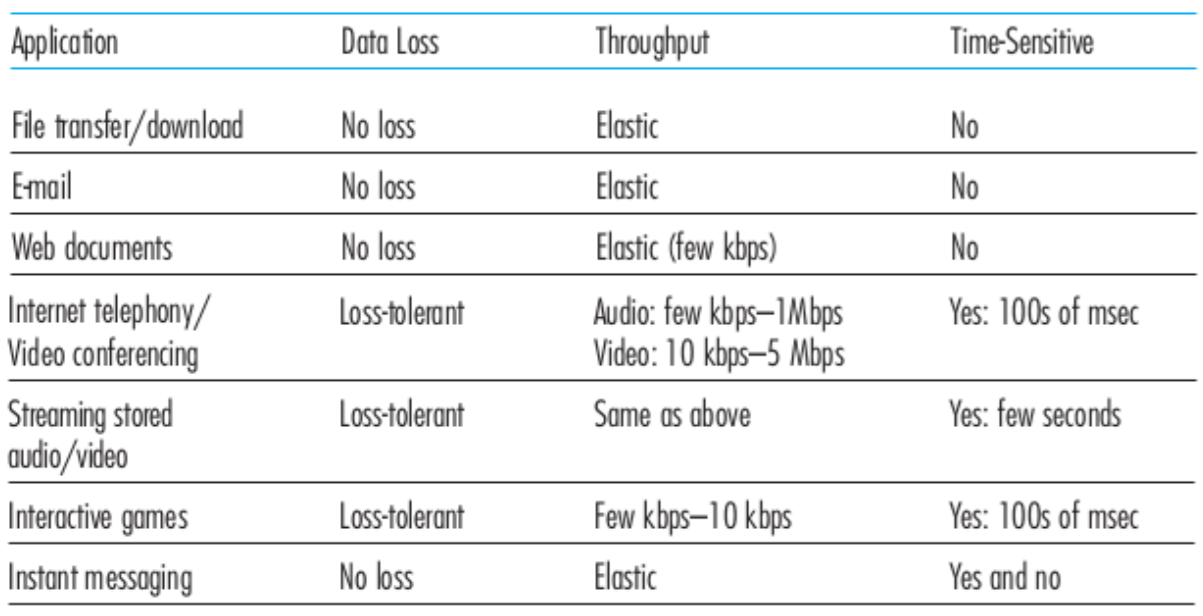
\includegraphics[width=12cm,height=4cm]{unit-17/figures/transport-service-requirements.png}
\end{table}

\subsubsection{Transmission Control Protocol (TCP)}

The Transmission Control Protocol (TCP) provides reliable transport between sending and receiving processes; the data received is identical to the data sent.
The protocol also provides flow control (so that the sender does not overwhelm the receiver) and congestion control (so that the sender is throttled when the network is overloaded).
The protocol does not provide a timing, minimum throughput guarantee or security --- these must be handled by the application layer.
TCP is a connection-oriented protocol; a connection must be set up between the client and the server before communication can occur.

\subsubsection{User Datagram Protocol (UDP)}

The User Datagram Protocol (UDP) provides unreliable data transfer between sending and receiving processes.
It does not provide reliability, flow control, congestion control, timing, throughput guarantee, security or connection setup.

UDP exists both because it is a very simple protocol to use and because it allows a lot more data to transferred across a network than TCP.
Data integrity is sacrificed for greater throughput.
This is useful for Internet telephony applications.

\begin{table}[htp]
  \centering
  \caption*{Application and transport protocols of common applications.}
  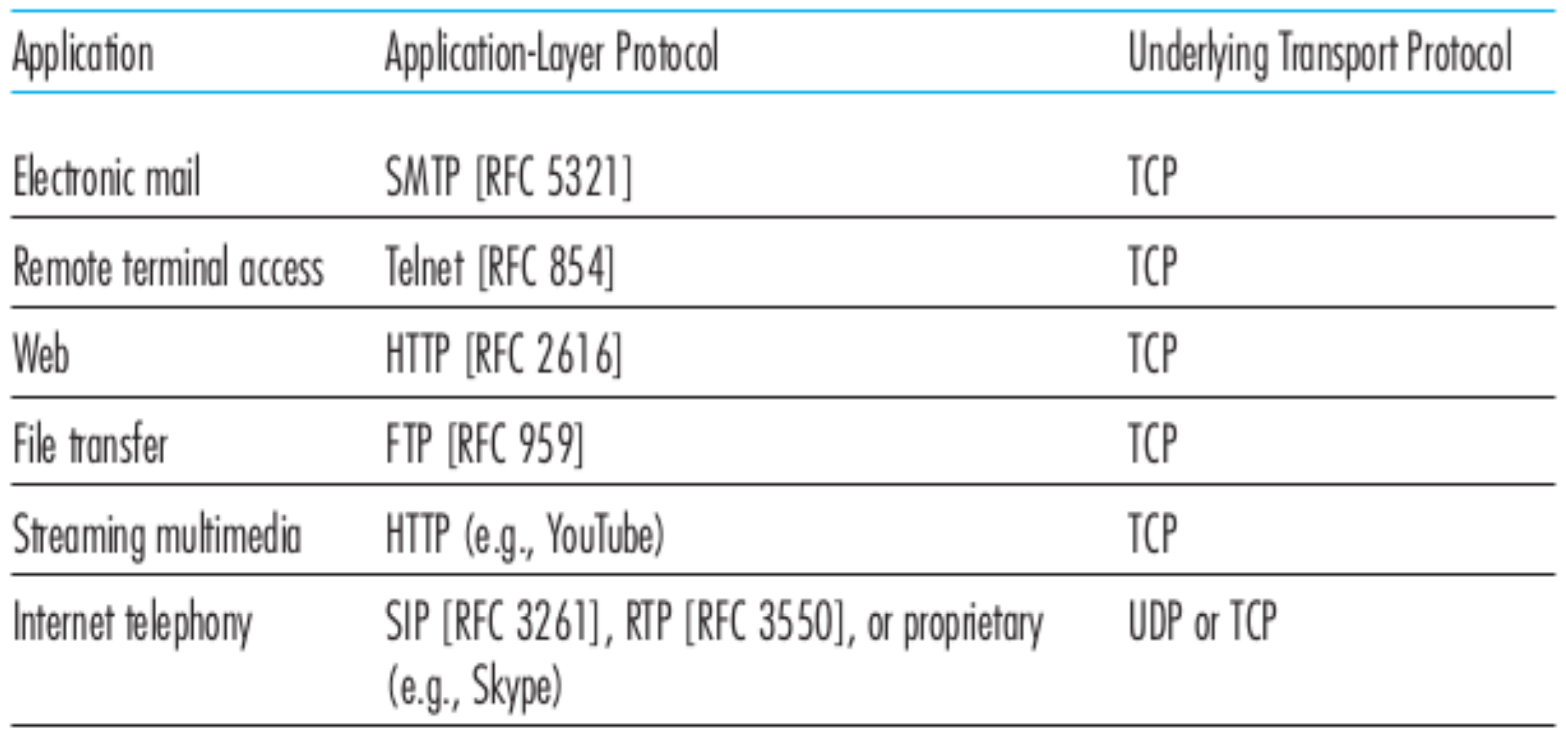
\includegraphics[width=12cm,height=4cm]{unit-17/figures/transport-protocols.png}
\end{table}

\subsection{Hypertext Transfer Protocol (HTTP)}

A web page consists of a base HTML file that may include several referenced objects, such as images, applets or media files.
Each object is addressable by a Uniform Resource Locator (URL), which consists of a host name and a path.

The Hypertext Transfer Protocol (HTTP) is the application layer protocol of the web.
The web uses a client-server architecture.
A web browser is a client that requests, receives and displays web objects.
The web server sends objects in response to requests.

HTTP uses the TCP protocol.
HTTP itself is a stateless protocol.
The server does not retain any information about past client requests.

\subsubsection{Non-Persistent HTTP}

\begin{enumerate}
  \item The HTTP client initiates a TCP connection to the HTTP server at the requested host address on port~\num{80}.
  \item The HTTP server accepts the connection and notifies the client.
  \item The HTTP client sends an HTTP request message (containing a URL to the requested object) through its TCP socket.
  \item The HTTP server receives the request message, forms a response message containing the requested object and sends its through its TCP socket.
  \item The HTTP waits until its message is received by the client, then closes the TCP connection.
  \item The HTTP client receives the response message and displays the HTML file.
  \item If object references are found in the HTML file, the above process is repeated for each object.
\end{enumerate}

The round-trip time (RTT) is the time it takes for a small packet to travel from the client to the server and back again.
The HTTP response time consists of one RTT to initiate the TCP connection, another RTT for the HTTP request to be sent and the HTTP response to start being received, and the file transmission time for the object being served.

\begin{equation*}
  \text{HTTP response time} = 2 \text{RTT} + \text{file transmission time}
\end{equation*}

\subsubsection{Persistent HTTP}

The use of non-persistent HTTP leads to a number of issues.
It takes two round-trips for each object and causes an OS overhead for each TCP connection.
Browsers often open parallel TCP connections to fetch referenced objects.

In persistent HTTP, the server leaves the connection open after sending a response.
Subsequent HTTP messages between the client and server are sent over an open connection.
This allows the client to send a request as soon as it encounters a referenced object.
This uses only one round-trip for each referenced object.

\subsubsection{HTTP Request Message}

HTTP messages are written in a human-readable ASCII format.
A request message begins with a request line, which contains the HTTP method (\texttt{GET}, \texttt{POST} or \texttt{HEAD}).
The request line is followed by header lines.
The end of the header is indicated by a carriage return and line feed (CRLF) at the start of a line.

\begin{figure}[htp]
  \centering
  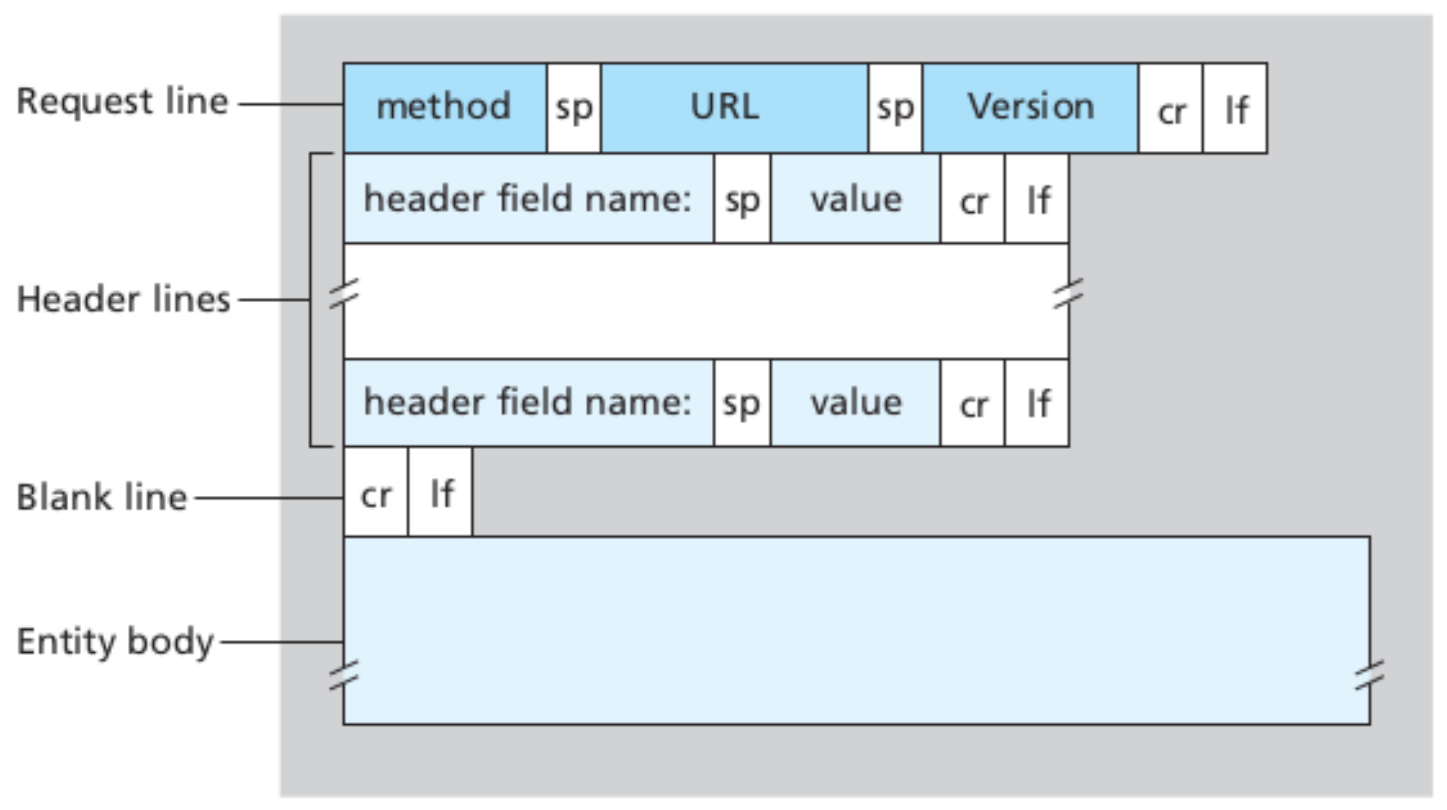
\includegraphics[width=12cm]{unit-17/figures/http-request.png}
  \caption*{General format of a HTTP request message.}
\end{figure}

\subsubsection{HTTP Response Message}

A response message begins with a status line, which contains the status code and status phrase.
Possible status codes and phrases include
\begin{itemize}
  \item 200 (OK) --- request succeeded, requested object contained in this message,
  \item 300 (Moved Permanently) --- requested object has moved to a new location specified in this message,
  \item 400 (Bad Request) --- request message not understood by server,
  \item 404 (Not Found) --- requested document not found on the server, and
  \item 505 (HTTP Version Not Supported).
\end{itemize}

The status line is followed by a header that ends with a CRLF at the start of a line.
The requested data follows the header.

\begin{figure}[htp]
  \centering
  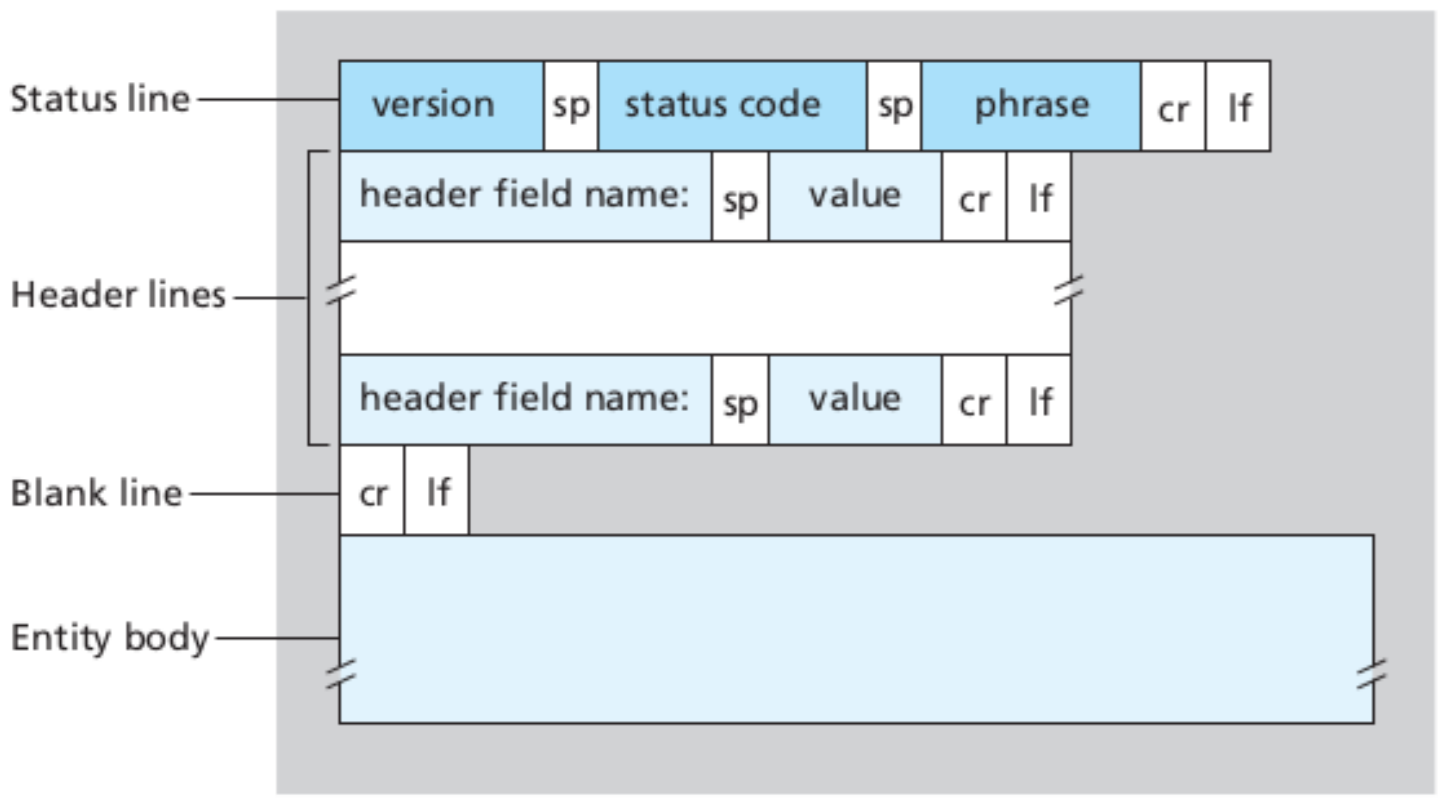
\includegraphics[width=12cm]{unit-17/figures/http-response.png}
  \caption*{General format of a HTTP response message.}
\end{figure}

\subsection{Simple Mail Transfer Protocol (SMTP)}

A user agent (UA) is an email client that is responsible for composing, editing and reading messages.
Incoming and outgoing messages are stored on a server.

A mail server contains mailboxes for each user that contain incoming messages and a message queue of outgoing messages.
The Simple Mail Transfer protocol (SMTP) is used to send email messages between mail servers.
A mail server takes on the role of client when it is sending emails, and the role of server when it is receiving emails.

SMTP uses TCP to reliably transfer emails directly from client to server at port~\num{25}.
An email transfer consists of three phases: handshake, transfer and closure.
SMTP uses a command and response interaction similarly to HTTP.
Commands and responses are written in ASCII text and responses contain status codes and phrases.
SMTP commands include \texttt{HELO}, \texttt{MAIL FROM}, \texttt{RCPT TO}, \texttt{DATA} and \texttt{QUIT}.

SMTP uses persistent connections.
It requires that messages are composed in \SI{7}{\bit} ASCII.
The end of a message is indicated by a CRLF followed by a period and another CRLF.
Whilst HTTP uses a ``pull'' interaction, SMTP uses a ``push'' interaction.
In HTTP, each object is encapsulated in its own response message.
In SMTP, multiple objects can be sent in multipart messages.

\subsection{Mail Access Protocols}

Whilst SMTP is used for delivering and storing messages to the mail server of a receiver, a mail access protocol is used for retrieving messages from a server.
\begin{itemize}
  \item POP3 (Post Office Protocol Version 3) --- authorisation and download
  \item IMAP (Internet Mail Access Protocol) --- more features, including manipulation of a stored message on a server
  \item HTTP (Hypertext Transfer Protocol)
\end{itemize}

POP3 uses an authorisation phase, in which client issues \texttt{user} and \texttt{pass} commands to declare a username and password, and a transaction phase, in which the client issues \texttt{list}, \texttt{retr}, \texttt{dele} and \texttt{quit} commands to list message numbers, retrieve a message by number, delete a message by number and quit the server.

POP3 download-and-delete mode deletes messages from the server once they are downloaded to the client.
They cannot be downloaded again on another client.
POP3 download-and-keep mode allows copies of messages on multiple clients.
POP3 is stateless across sessions.

IMAP keeps all messages on the server and allows messages to be organised in folders.
IMAP retains the user state across sessions.
This includes the names of folders and the mappings of message identifiers to folder names.

\subsection{Domain Name System (DNS)}

Internet hosts and routers have \SI{32}{\bit} IP addresses used for addressing datagrams, and hostnames that are used by humans.
A Domain Name System (DNS) is a distributed database that maps hostnames to IP addresses.

A DNS provides
\begin{itemize}
  \item hostname to IP address translation,
  \item host aliasing (allows a host with a single canonical name to have multiple alias names),
  \item mail server aliasing, and
  \item load distribution (web servers are replicated such that many IP addresses correspond to one host name).
\end{itemize}

DNS is an application layer protocol used by hosts and name servers to communicate to resolve names.
DNS servers are end systems that exist at the network edge.
Lookup is performed as close as possible to the source host using a local DNS server.

A single centralised DNS does not exist as this would introduce a single point of failure.
It would also be impossible to implement as all Internet traffic would have to pass through a single server.
There would be long delays for end systems far from the server, and performing maintenance on the server would cause all Internet services to stop.

\subsubsection{The DNS Distibuted Hierarchical Database}

DNS is implemented using a hierarchy of many name servers.

\begin{figure}[htp]
  \centering
  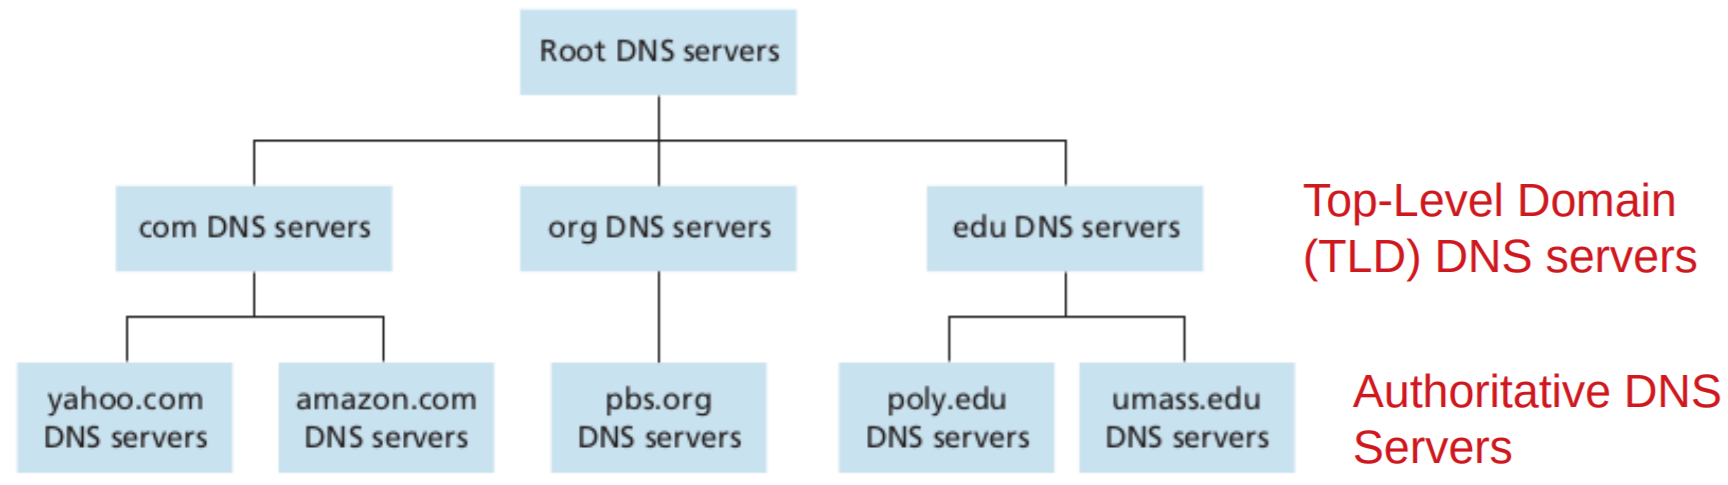
\includegraphics[width=15cm]{unit-17/figures/dns-hierarchy.png}
  \caption*{A portion of the hierarchy of DNS servers.}
\end{figure}

There are several root DNS servers worldwide.
Each is actually a network of replicated servers.
A top-level domain (TLD) server is responsible for \texttt{com}, \texttt{org}, \texttt{net}, \texttt{edu}, \texttt{gov} and all top-level country domains.
An authoritative server is a DNS server owned by an organisation.
It provides authoritative hostname to IP mappings for the named hosts of the organisation.
These can be maintained by the organisation itself or a service provider on its behalf.

Each ISP has its own local DNS server, which is also known as a `default name server'.
Local DNS servers do not strictly belong to the DNS hierarchy.
When a host makes a DNS query, the query is sent to the local DNS server, which maintains a cache of recent name to address mappings (that may be out of date).
It also acts as a proxy and forwards the query into the hierarchy if necessary.

\subsubsection{DNS Resolution}

With an iterative DNS query, if a contacted server does not know the mapping of a host name, it will respond with the name of server that might know.
For example, a local DNS server may query the root DNS server, which may respond with the name of the TLD server.
The local DNS server then queries the TLD server and receives the name of an authoritative server.
When the local DNS server queries the authoritative server, it will return the address of the requested host.

With a recursive query, each contacted server resolves the name itself instead of returning a reference to next server.
This may not be desirable as it can place a heavy load on the upper levels of the DNS hierarchy.

\subsubsection{DNS Caching and Records}

Once a name server learns a mapping, it stores that mapping in cache.
Cache entries timeout after a period of time known as a `time-to-live' (TTL).
TLD mappings are typically cached in local DNS servers.
This means that root servers are not visited often.
A cached entry may be out of date.
If a host changes its IP address, it may not be known Internet-wide until all of its cached mappings have expired.

DNS records are stored in the distributed database as resource records (RR), which consist of a name, value, type and TTL.
\begin{itemize}
  \item Type A
  \begin{itemize}
    \item Name is the host name
    \item Value is the IP address
  \end{itemize}
  \item Type CNAME
  \begin{itemize}
    \item Name is an alias for a canonical name
    \item Value is the canonical name
  \end{itemize}
  \item Type NS
  \begin{itemize}
    \item Name is a domain name
    \item Value is the host name of the authoritative server for the domain
  \end{itemize}
  \item Type MX
  \begin{itemize}
    \item Value is the name of the mail server associated with name
  \end{itemize}
\end{itemize}

\subsubsection{DNS Protocol Messages}

DNS queries and replies follow the same format.
The message header contains a \SI{16}{\bit} identification number for the query.
The same number is used for a reply to that query.
The flags state whether the message is a query or reply, whether recursion is desired, whether recursion is available and whether the reply is authoritative.

\begin{figure}[htp]
  \centering
  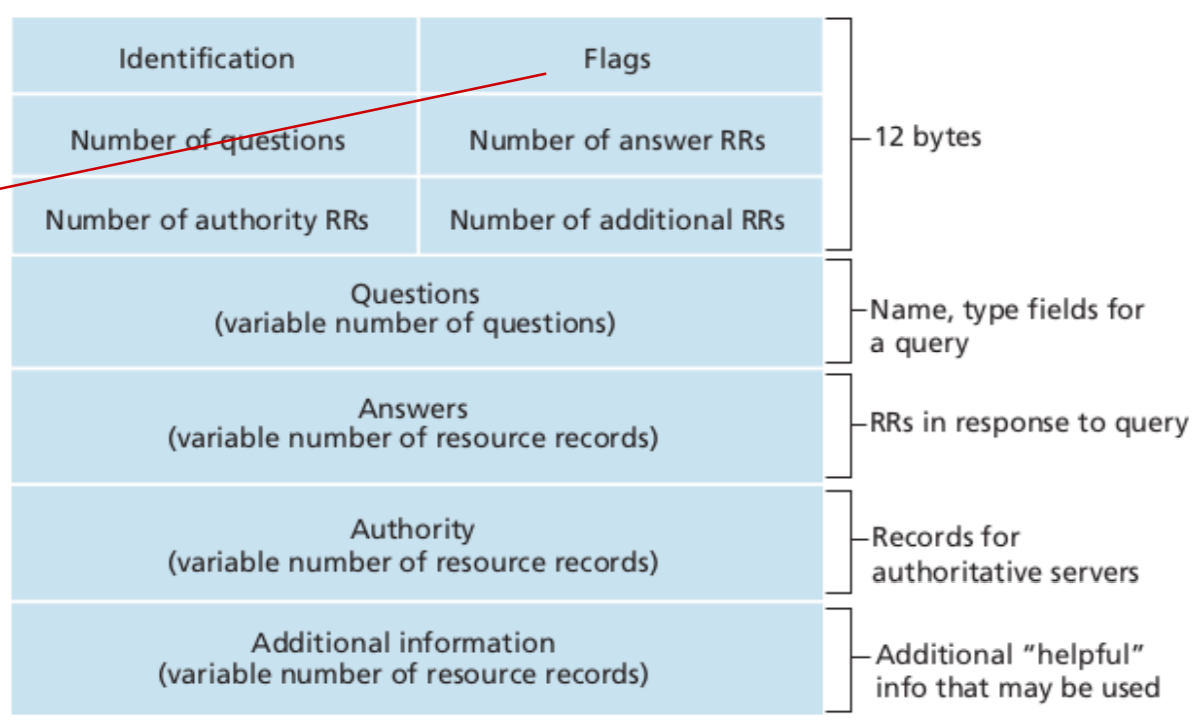
\includegraphics[width=12cm]{unit-17/figures/dns-message.png}
  \caption*{The general format of a DNS query or response message.}
\end{figure}

\subsubsection{DNS Registration}

When an organisation registers its host name \texttt{example.com} with a DNS registrar, the registrar inserts two RRs into the relevant TLD server.
These are a type~NS record for the name of the authoritative server of the organisation (\texttt{example.com}, \texttt{dns.example.com}, NS) and a type~A record for the IP address of the authoritative server (\texttt{dns.example.com}, \texttt{111.111.111.1}, A).
The authoritative server contains type~A records for its subdomains and a type~MX record for its mail server.
